\documentclass[11pt]{article}
% Shared preamble for the report (XeLaTeX). Fonts ship with TeX Live / MacTeX.
\usepackage[letterpaper,margin=1in,headsep=0.3in,footskip=0.4in]{geometry}
\usepackage{fontspec}
\usepackage{unicode-math}
\setmainfont{TeX Gyre Termes}
\setsansfont{TeX Gyre Heros}[Scale=MatchLowercase]
\setmonofont{DejaVu Sans Mono}[Scale=0.82]
\setmathfont{TeX Gyre Termes Math}
\usepackage{microtype}
\linespread{1.0}
\emergencystretch=1.5em
\setlength{\parindent}{1.4em}
\setlength{\parskip}{0pt}
\frenchspacing
\widowpenalty=10000 \clubpenalty=10000

% colours
\usepackage{xcolor}
\definecolor{linkblue}{HTML}{1A4F8B}
\definecolor{muted}{HTML}{5B6270}
\definecolor{rule}{HTML}{9AA1AC}

% headings: numbered, bold, as in HW5
\usepackage{titlesec}
\titleformat{\section}{\normalfont\fontsize{12}{14}\bfseries}{\thesection.}{0.5em}{}
\titleformat{\subsection}{\normalfont\normalsize\bfseries}{\thesubsection}{0.6em}{}
\titleformat{\subsubsection}[runin]{\normalfont\normalsize\bfseries}{}{0em}{}[.]
\titlespacing*{\section}{0pt}{14pt plus 3pt minus 2pt}{6pt plus 1pt}
\titlespacing*{\subsection}{0pt}{10pt plus 2pt minus 2pt}{4pt plus 1pt}
\titlespacing*{\subsubsection}{0pt}{6pt plus 2pt}{0.6em}
\newcommand{\para}[1]{\par\smallskip\noindent\textbf{#1}\hspace{0.5em}}

% lists
\usepackage{enumitem}
\setlist{itemsep=2pt,parsep=0pt,topsep=4pt,leftmargin=1.6em}

% tables and figures
\usepackage{booktabs,threeparttable,makecell,multirow,array,tabularx}
\renewcommand{\arraystretch}{1.12}
\setlength{\aboverulesep}{0.3ex}\setlength{\belowrulesep}{0.5ex}
\usepackage{graphicx}
\usepackage{flafter}  % floats never precede their first mention
\usepackage[labelfont=bf,labelsep=period,font=small,justification=justified,
            singlelinecheck=false,skip=5pt]{caption}
\captionsetup[table]{position=top}
\renewcommand{\TPTnoteSettings}{\setlength\leftmargin{0pt}\setlength\labelwidth{0pt}\setlength\labelsep{0pt}\setlength\itemsep{1pt}}
\setlength{\textfloatsep}{14pt plus 3pt minus 3pt}
\setlength{\floatsep}{12pt plus 3pt minus 3pt}
\renewcommand{\topfraction}{0.9}\renewcommand{\bottomfraction}{0.6}
\renewcommand{\textfraction}{0.1}\renewcommand{\floatpagefraction}{0.8}

% running head and page numbers
\usepackage{fancyhdr}
\pagestyle{fancy}
\fancyhf{}
\renewcommand{\headrulewidth}{0pt}
\fancyhead[R]{\footnotesize\color{muted}\shorttitle}
\fancyfoot[C]{\small\thepage}
\fancypagestyle{plain}{\fancyhf{}\renewcommand{\headrulewidth}{0pt}\fancyfoot[C]{\small\thepage}}

% references and links
\usepackage[numbers,square,sort&compress]{natbib}
\setlength{\bibsep}{2pt plus 1pt}
\renewcommand{\bibfont}{\small}
\usepackage[colorlinks=true,linkcolor=linkblue,citecolor=linkblue,urlcolor=linkblue]{hyperref}
\usepackage[nameinlink,capitalise,noabbrev]{cleveref}
\crefname{table}{Table}{Tables}
\crefname{figure}{Figure}{Figures}

% title block
\newcommand{\shorttitle}{}
\newcommand{\papertitle}[1]{\def\@ptitle{#1}}
\makeatletter
\newcommand{\maketitleblock}[4]{% title, author line, info line, abstract
  \thispagestyle{plain}
  \begin{center}
    {\fontsize{16.5}{20}\selectfont\bfseries #1\par}
    \vspace{9pt}
    {\normalsize #2\par}
    \vspace{2pt}
    {\small\color{muted}#3\par}
  \end{center}
  \vspace{4pt}
  \begin{center}\textbf{Abstract}\end{center}
  \vspace{-4pt}
  {\small\leftskip=0.45in\rightskip=0.45in\noindent #4\par}
}
\makeatother
\newcommand{\keywords}[2]{%
  \vspace{5pt}
  {\small\leftskip=0.45in\rightskip=0.45in\noindent\textit{Keywords:} #1\par
   \noindent\textit{JEL codes:} #2\par}
  \vspace{6pt}{\centering\color{rule}\rule{0.35\textwidth}{0.4pt}\par}\vspace{2pt}}

\renewcommand{\shorttitle}{Unexplained Pessimism Ahead of the 2026 Midterms}
% Public replication repository:
\newcommand{\repourl}{\url{https://github.com/JonasWooh/unexplained-pessimism}}

\begin{document}

\maketitleblock
{Unexplained Pessimism:\\Economic Fundamentals, Media Narratives, and\\U.S.\ Consumer Sentiment Ahead of the 2026 Midterms}
{Jonas Wu (jw9452)}
{AI Applications in Finance, Final Project\\Data cutoff: October 16, 2026\\Project repository: \repourl}
{U.S. consumer sentiment has stayed far below the level implied by headline economic indicators. Using the real-time vintages of unemployment, PCE inflation and real GDP growth available at each survey date, we fit an economic-only model to the Michigan Index of Consumer Sentiment over 2010–2019 and define the sentiment gap as its out-of-sample residual. The gap averages −35.8 points in 2025 and −39.8 in 2026, and the three indicators account for only 7–11\% of the decline since 2019. We code a documented news and social-media corpus with a large language model validated against 360 items labeled by two independent annotators (tone $\kappa = 0.73$, against 0.79 between annotators and 0.35 for a finance dictionary); swapping political names does not detectably change the coding. Lagged news tone improves forecasts over the economic-only model ($p = 0.041$) but not once household-pressure and political controls are added ($p = 0.23$; none of 20 specifications significant), and accounts for at most about 5\% of the gap. The gap is similar across demographic groups, widens within the web-only survey period and predates the campaign. Media bias is not the main explanation; we propose a randomized framing experiment for causal identification.}
\keywords{consumer sentiment; real-time data; media bias; large language models; forecasting; 2026 midterm elections}{D12, D84, E71, C53}

% ======================================================================
\section{Introduction}\label{sec:intro}

Since mid-2021, U.S. consumers have reported far gloomier views of the economy than unemployment, inflation and output growth would suggest. A gap of this kind admits three readings. Consumers may be responding to pressures that headline indicators miss, such as the level of prices or the cost of borrowing (H1). Their perceptions may reflect selective information, framing or cognitive bias, possibly transmitted through news and social media (H2). Or the discrepancy may be an artifact of measurement, timing or an incomplete model (H3). The three are not exclusive. We treat each as a hypothesis, test what the data allow, and report where they cannot discriminate.

\Cref{sec:baseline} measures how much of the gap unemployment, inflation and GDP growth explain (RQ3) and tests H1 and H3. \Cref{sec:corpus,sec:measure} build and validate the media measures and benchmark candidate biases (RQ1). \Cref{sec:forecast,sec:causal} test forecasting value (RQ5) and timing and causal reasoning (RQ2), \cref{sec:mech} covers perceptual mechanisms (RQ4), heterogeneity, survey mode and the election period, and \cref{sec:falsify} applies pre-registered falsification criteria (RQ6).

The design, including the models, the primary media hypothesis and the falsification criteria with their decision rules, was frozen before any model was estimated; all 150 specifications run, including unfavorable ones, are registered and deviations are logged (\cref{app:repro}). Data end on October 16, 2026, so the October Michigan reading is preliminary; the election is on November 3.

In brief, the gap is large, robust and unexplained by fundamentals, survey mode, partisan composition or the election calendar, and media tone adds no out-of-sample information once household and political controls are included. We read this as a negative result for the media-bias explanation, not as evidence that the remaining pessimism is irrational.

% ======================================================================
\section{The real-time economic baseline}\label{sec:baseline}

\subsection{Data and timing}
Sentiment is the University of Michigan Index of Consumer Sentiment (ICS) and its two components, Current Economic Conditions (ICC) and Consumer Expectations (ICE). Michigan asks about personal finances, business and buying conditions, not about the three statistics themselves. For each survey month $t$ we take the seasonally adjusted U-3 unemployment rate, headline PCE inflation computed as $100 \times (P_t/P_{t-12} - 1)$ within a single vintage of the PCE price index, and real GDP growth from the ALFRED vintage available on the first day of $t$ \citep{croushore2001,alfred}. GDP growth is the latest published quarter-over-quarter annualized rate, held until the next release and never interpolated (year-over-year growth is a robustness check). The economic-only model is
\begin{equation}
  \mathit{ICS}_t = \alpha + \beta_u U^{\mathrm{rt}}_t + \beta_\pi \pi^{\mathrm{rt}}_t + \beta_g g^{\mathrm{rt}}_t + \textstyle\sum_{m} \delta_m D_{mt} + \varepsilon_t ,
  \label{eq:m1}
\end{equation}
estimated on 2010–2019 with Newey–West standard errors \citep{newey1987}; month dummies were retained by a pre-registered joint test ($p = 0.001$). The sentiment gap is $\mathit{ICS}_t - \widehat{\mathit{ICS}}_t$ for every month from 2020 on. A negative gap is pessimism that M1 cannot explain, not evidence of perceptual bias. Prediction intervals come from a moving-block bootstrap of in-sample residuals \citep{kunsch1989}.

\subsection{How large is the gap?}
M1 fits the estimation window closely ($R^2 = 0.90$, $n = 120$; unemployment $-4.84$, s.e.\ 0.29; inflation $-2.31$, s.e.\ 1.00; GDP growth 1.09, s.e.\ 0.28), and its residuals are stationary. \Cref{fig:gap} and \cref{tab:gap} show the result. During the pandemic the indicators leave the estimation range (unemployment 14.7\%, GDP growth $-32.9\%$ and $+33.1\%$ annualized), the monthly error has a root mean square of 30.3, and these months are not interpreted. From the second half of 2021 a negative gap opens and widens to $-35.8$ in 2025 and $-39.8$ in 2026, far outside the 95\% band of M1's prediction error; after 2022 the fundamentals account for only 7–11\% of the decline since 2019. Inflation lowered predicted sentiment by 9.4 points in 2021–2022 and unemployment by 2.6; in 2025–2026 no indicator contributes more than 4.2 points. The current-conditions component is always further below its prediction than the expectations component.

\begin{table}[htbp]
\centering
\begin{threeparttable}
\caption{\textbf{Sentiment gap relative to the economic-only model (M1), by period}}
\label{tab:gap}
\small
\begin{tabular}{@{}l r r r c r r r@{}}
\toprule
 & & \multicolumn{4}{c}{Index of Consumer Sentiment (ICS)} & \multicolumn{2}{c}{Mean gap}\\
\cmidrule(lr){3-6}\cmidrule(l){7-8}
Period & Months & \makecell[r]{Actual\\change} & \makecell[r]{Mean\\gap} & \makecell{95\% band\\under M1} & \makecell[r]{Explained\\share $S$} & ICC & ICE\\
\midrule
2021-07 to 2022-12 & 18 & −32.6 & −22.9 & [−7.7, 7.9] & 0.30 & −35.0 & −15.2 \\
2023-01 to 2024-12 & 24 & −27.0 & −25.2 & [−4.4, 4.7] & 0.07 & −39.8 & −15.8 \\
2025-01 to 2025-12 & 12 & −38.4 & −35.8 & [−4.2, 3.9] & 0.07 & −47.7 & −28.2 \\
2026-01 to 2026-10 & 10 & −44.8 & −39.8 & [−5.3, 5.1] & 0.11 & −55.2 & −29.9 \\
\bottomrule
\end{tabular}
\begin{tablenotes}[flushleft]\footnotesize
\item \textit{Notes:} Changes are relative to the 2019 average. Gap = actual − M1 out-of-sample prediction; M1 regresses each index on real-time U-3 unemployment, PCE inflation (year over year) and real GDP growth (quarter over quarter, annualized), fitted on 2010–2019 with month dummies. The band is the 95\% range of the period-mean prediction error under M1 (moving-block bootstrap, block length 12, 2,000 draws); every period mean lies outside it ($p < 0.001$). $S = 1 - \text{mean gap}/\text{actual change}$, the share of the decline since 2019 that M1 accounts for. ICC = Current Economic Conditions; ICE = Consumer Expectations. Pandemic months (2020-01 to 2021-06) are omitted. 2026-10 is the preliminary reading.
\item \textit{Source:} \texttt{results/stage1\_m1/m1\_periods.csv}.
\end{tablenotes}
\end{threeparttable}
\end{table}


\begin{figure}[htbp]
  \centering
  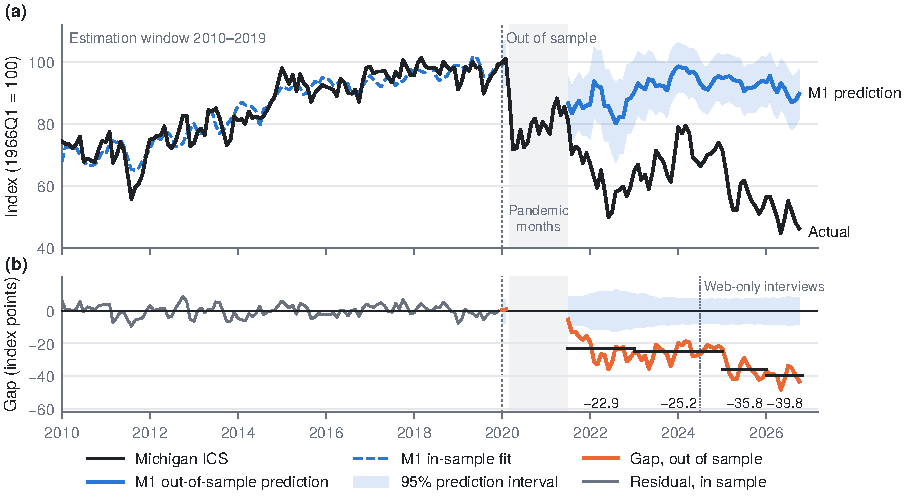
\includegraphics[width=\textwidth]{figures/fig_gap.pdf}
  \caption{\textbf{Michigan sentiment against the economic-only prediction.} Panel (a) shows the ICS and the M1 prediction from \cref{eq:m1}; the dashed line is the 2010–2019 in-sample fit and the band is the 95\% moving-block bootstrap prediction interval. Panel (b) shows the gap; horizontal segments and labels give the period means in \cref{tab:gap}. Pandemic months (shaded) are not interpreted because the indicators leave the estimation range. The dotted line marks the first month of web-only interviewing (July 2024). Source: \texttt{results/stage1\_m1/m1\_gap\_monthly.csv}.}
  \label{fig:gap}
\end{figure}

\subsection{Alternative explanations}
\Cref{tab:alt} reports the pre-registered checks of H1 and H3.

\begin{table}[htbp]
\centering
\begin{threeparttable}
\caption{\textbf{Alternative explanations of the gap: household pressure, estimation window and measurement}}
\label{tab:alt}
\footnotesize
\begin{tabular}{@{}l c c c l@{}}
\toprule
 & \multicolumn{3}{c}{Mean ICS gap} & \\
\cmidrule(lr){2-4}
Specification & 2021-07 to 2022-12 & 2025 & 2026-01 to 2026-10 & Test \\
\midrule
\multicolumn{5}{@{}l}{\textit{A. Household pressure (H1), pre-registered}}\\
M1, 2010-06 to 2019-12 & −23.1 & −35.9 & −39.9 &  \\
\quad + 36-month cumulative PCE inflation & −22.4 & −34.9 & −39.1 & $p = 0.79$ \\
\quad + 30-year mortgage rate & −23.2 & −35.2 & −39.3 & $p = 0.78$ \\
\quad + real disposable income per capita & −21.5 & −36.0 & −39.7 & $p = 0.28$ \\
\quad + gasoline price & −22.6 & −35.4 & −38.8 & $p = 0.32$ \\
\quad + all four household variables & −21.6 & −35.5 & −38.5 & $p = 0.24$ to $0.89$ \\
\addlinespace
\multicolumn{5}{@{}l}{\textit{B. Estimation window (H3c)}}\\
2000-09 to 2019-12, fully real time & −10.1 & −31.7 & −33.0 &  \\
\quad + 36-month cumulative PCE inflation\textsuperscript{a} & −11.3 & −26.2 & −30.7 & $p = 0.008$ \\
1978-01 to 2019-12, quasi real time & −25.1 & −35.9 & −40.3 &  \\
Expanding window, re-estimated monthly & & −25.2 & & \\
\addlinespace
\multicolumn{5}{@{}l}{\textit{C. Measurement (H3a, H3b): estimated effect on the gap}}\\
Web-interview step from 2024-07, ICS & \multicolumn{3}{c}{−5.7 [−11.9, 0.5]} & $p = 0.072$ \\
Web-interview step from 2024-07, ICC & \multicolumn{3}{c}{−8.0 [−11.9, −4.1]} & $p < 0.001$ \\
Web-interview step from 2024-07, ICE & \multicolumn{3}{c}{−4.1 [−12.3, 4.0]} & $p = 0.32$ \\
Republican share lower by 2 to 6 points, ICS & \multicolumn{3}{c}{−0.8 to −2.7} & $\leq$ 7\% of gap \\
\bottomrule
\end{tabular}
\begin{tablenotes}[flushleft]\footnotesize
\item \textit{Notes:} Panels A and B report the mean out-of-sample ICS gap. In Panel A the household variables are added to M1 and the model is estimated on 2010-06 to 2019-12, the first month with real-time income data, so the baseline differs slightly from \cref{tab:gap}. Test: HAC $p$-value of the added variable(s). Panel C, first three rows: coefficient on a step dummy for web-only interviewing in a regression of the 2023--2025 monthly gap, with 95\% confidence interval. Last row: change in the 2025--2026 ICS if the Republican share of respondents were 2, 4 or 6 points lower, using estimated group shares (Democrats 0.26, independents 0.54, Republicans 0.20). \textsuperscript{a}Exploratory, not pre-registered.
\item \textit{Source:} \texttt{results/stage1\_h1/h1\_models\_with\_exploratory.csv}, \texttt{stage1\_windows/m1\_windows.csv}, \texttt{stage1\_m1/m1\_recursive\_expanding.csv}, \texttt{stage1\_h3/h3a\_mode.csv}, \texttt{stage1\_h3/h3b\_composition\_bound.csv}.
\end{tablenotes}
\end{threeparttable}
\end{table}


\para{Household pressure (H1).} Adding 36-month cumulative PCE inflation, the 30-year mortgage rate, real disposable income per capita or the gasoline price, singly or together, barely moves the gap, and none of the coefficients is significant. This is a failure of identification, not evidence of absence: 89\% of out-of-sample cumulative-inflation values and 96\% of mortgage-rate values lie outside their 2010–2019 range. In an exploratory window from 2000, cumulative inflation is significant and shrinks the gap since 2021 by about 24\% ($-20.4$ to $-15.5$). H1 remains open.

\para{Model and window (H3c).} The 2021–2022 gap is window-sensitive ($-10.1$ to $-25.1$) because the inflation coefficient is poorly identified when inflation barely varies. The 2025 gap is not: $-31.7$ to $-35.9$ across fixed windows, $-25.2$ even when re-estimated monthly, and $-35.5$ to $-36.3$ across HAC lags, seasonal terms, GDP definition and cutoff date.

\para{Measurement (H3a, H3b).} Web interviewing coincides with a step of about $-8$ points in ICC but no stable step in ICS or ICE. Partisan reactions to the 2025 change of administration are large and opposite (Democrats $-28.2$, Republicans $+17.6$), yet Republicans in 2025 were also 29.3 points below their own 2017–2019 level, and a plausible composition shift moves the ICS by at most 2.7 points.

\subsection{Why falling inflation need not end concern about prices}
Inflation is a rate of change; the price level it leaves behind is permanent. With inflation near 3\% in 2025–2026, 36-month cumulative PCE inflation was still 9.4\% (5.3\% in 2019), and a household comparing today's prices with remembered ones sees no relief from disinflation. Michigan's open-ended reasons are consistent with this: the share saying their finances worsened because of high prices was 7.3\% in 2019, 39.8\% in 2022 and 44.8\% in 2025–2026, even though inflation in the last period was less than half its 2022 rate (\cref{sec:mech}). Aggregate GDP growth can likewise diverge from household experience: it includes investment, government spending and net exports, its gains are unevenly distributed, and borrowing costs for homes and cars have roughly doubled since 2021. These arguments make H1 plausible; \cref{tab:alt} shows that our sample cannot estimate its size.

% ======================================================================
\section{A documented media corpus}\label{sec:corpus}

\para{Sources and selection.} \Cref{tab:corpus} summarizes the corpus. National news comes from the full NYT and Guardian archives, the national sources that are free, reproducible and reach back to 2010; Media Cloud supplies random-day samples of national and local outlets for 2025–2026. Social media are YouTube comments on ten news channels (YouTube is the platform most used by U.S. adults) and four Reddit communities, which skew young and educated. Items enter if their text matches one of 26 economic search terms (prices, jobs, growth and recession, rates and housing, general economy) and were published from January 1, 2010 to October 14, 2026.

\para{Units, duplicates and missing data.} Units differ by source (\cref{tab:corpus}). Matching on normalized URLs, text and MinHash near-duplicates flags 2,484 duplicates and 21,188 reposts; local news shrinks from 25,055 items to 7,264 once wire copies are removed, so repost counts measure supply amplification. Advertisements (8) and obituaries (170) are excluded. Account fields were not stored, by privacy design, so automated accounts cannot be identified. Gaps are reported, not filled: the NYT archive returns nothing for January 8–31, 2026 and stops on October 4; GDELT and outlet-slant ratings were unavailable.

\para{Supply, engagement and exposure.} The corpus measures content supply. Likes and replies are archived snapshots, used only descriptively; they show attention on a platform, not what respondents saw. The only exposure-side evidence is Michigan's question on whether respondents heard favorable or unfavorable news (\cref{sec:causal}).

\para{Coding sample.} Keyword precision against the gold standard is 0.98 for the Guardian but 0.59 for the NYT and 0.47 for Reddit, so every index first filters on the LLM's relevance judgment. The LLM coded a stratified sample of 11,431 items with known inclusion probabilities, including 40 national items per month (about 26 relevant); indices are weighted ratio estimates over relevant items.

\begin{table}[htbp]
\centering
\begin{threeparttable}
\caption{\textbf{Corpus composition}}
\label{tab:corpus}
\footnotesize
\setlength{\tabcolsep}{4pt}
\begin{tabular}{@{}l l l l r r r@{}}
\toprule
Source & Unit & Design & Coverage & Items & Coded & Relevant\\
\midrule
\multicolumn{7}{@{}l}{\textit{National news (main media measure)}}\\
New York Times & Abstract and lead & Full archive & 2010-01 to 2026-10 & 38,468 & 7,222 & 4,540\\
Guardian (U.S. economy) & Full text & Full archive & 2010-01 to 2026-10 & 4,286 & 849 & 735\\
\addlinespace
\multicolumn{7}{@{}l}{\textit{Comparison sources (recent periods only)}}\\
Media Cloud, national & Headline & Random days & 13 months, 2025–26 & 3,854 & 260 & 178\\
Media Cloud, state and local & Headline & Random days & 19 months, 2025–26 & 25,055 & 760 & 593\\
Reddit (4 communities) & Post & Random days or months & 2010-01 to 2026-10 & 41,096 & 1,420 & 775\\
YouTube (10 news channels) & Comment & Non-probability & 2023-01 to 2026-10 & 54,659 & 920 & 860\\
\midrule
Total & & & & 167,418 & 11,431 & 7,681\\
\bottomrule
\end{tabular}
\begin{tablenotes}[flushleft]\footnotesize
\item \textit{Notes:} Items are keyword-matched units before de-duplication. Coded items are the stratified sample labeled by the LLM; relevant items are those it judged to concern the U.S. economy (23 ``unsure'' items are excluded from all indices). Reddit sampling started in 2015 for r/economy and r/Economics and covers 2010 onward for r/personalfinance and r/inflation. YouTube videos were selected by date coverage, so its comments carry no sampling weights.
\item \textit{Source:} \texttt{corpus/corpus\_documentation.md}; \texttt{labels/ai\_corpus\_labels.csv}.
\end{tablenotes}
\end{threeparttable}
\end{table}

% ======================================================================
\section{Measuring coverage with AI}\label{sec:measure}

\subsection{Codebook and human gold standard}
The codebook was written before any model was applied (\cref{app:codebook}). After a relevance judgment it records five dimensions: tone, with factual direction and emotional intensity coded separately from wording; selection and salience (13 topics); framing (price level or inflation rate, household or national, current or forecast); factual calibration; and political attribution, with the explicit rule that criticism is not bias. Two annotators labeled a stratified sample of 360 items independently, after 30 calibration items and without AI assistance; 593 item-dimension disagreements were adjudicated with written reasons. Agreement is high for relevance ($\kappa = 0.81$), tone (0.79) and price framing (0.93), and weakest for emotional intensity (0.59) \citep{cohen1960}. The gold standard was split into 100 development and 260 test items.

\subsection{LLM coding and validation}
Coding used one fixed model in the Codex command-line tool (GPT-6 Luna, high reasoning effort; temperature cannot be set), run in an isolated folder holding only the prompt and inputs. Two prompts were compared on the development set (mean $\kappa$ 0.652 and 0.670); the second was frozen and scored once on the test set. All 1,315 evidence excerpts returned on the test set appear verbatim in the source, and a re-run of 26 items reproduces relevance in 92\% and tone in 85\% of cases.

In \cref{tab:ai} the LLM's agreement with the gold standard approaches the agreement between the two humans (relevance 0.86 against 0.81, tone 0.73 against 0.79, price framing 0.83 against 0.93) and is much higher than the Loughran–McDonald dictionary \citep{loughran2011}, VADER \citep{hutto2014}, keyword rules or a TF-IDF classifier on every dimension where they apply (all paired bootstrap differences in macro-F1 exclude zero). Keyword rules fail on the two topics at the heart of the inflation narrative (rising prices $\kappa = 0.10$, easing inflation $-0.01$), and the dictionary's tone accuracy collapses outside national news ($\kappa$ 0.51 national, 0.19 local, 0.10 social). A classifier trained on the 100 human development labels is the worst method, so a small human sample cannot replace the coder. Weaker dimensions, listed in the table notes, serve only as secondary or descriptive measures.

\begin{table}[htbp]
\centering
\begin{threeparttable}
\caption{\textbf{Agreement with the human gold standard: LLM coding against low-cost baselines}}
\label{tab:ai}
\footnotesize
\begin{tabular}{@{}l r c c c c c c c@{}}
\toprule
 & & Human & & \multicolumn{2}{c}{Dictionary} & & \multicolumn{2}{c}{TF-IDF + logit} \\
\cmidrule(lr){5-6}\cmidrule(l){8-9}
Dimension & $n$ & A vs.\ B & LLM [95\% CI] & LM & VADER & Keyword & \makecell{LLM\\labels} & \makecell{100 human\\labels} \\
\midrule
Relevance (yes/no) & 236 & 0.81 & 0.86 [0.78, 0.92] & -- & -- & 0.00 & 0.74 & 0.41 \\
Tone & 174 & 0.79 & 0.73 [0.63, 0.81] & 0.35 & 0.27 & -- & 0.39 & 0.13 \\
Price framing & 174 & 0.93 & 0.83 [0.75, 0.90] & -- & -- & 0.48 & 0.64 & 0.39 \\
Topics (mean of 13) & 174 & -- & 0.79 & -- & -- & 0.58 & 0.69 & 0.23 \\
\bottomrule
\end{tabular}
\begin{tablenotes}[flushleft]\footnotesize
\item \textit{Notes:} Cohen's $\kappa$ against the adjudicated gold standard on the 260-item test set, scored once after the prompt was frozen on the 100-item development set. Relevance is scored on items whose gold label is yes or no; the other dimensions on the 174 items that both the gold standard and the LLM judge relevant. Human A vs.\ B is the agreement between the two independent annotators on all 360 items. LM = Loughran--McDonald; dictionary thresholds were set on the development set. The keyword rule marks every item relevant, so its relevance $\kappa$ is zero. Confidence intervals are percentile bootstrap. Dimensions without a low-cost baseline, LLM $\kappa$ (human A vs.\ B in parentheses): factual direction 0.57 (0.72); numeric claim 0.79 (0.86); perspective 0.63 (0.78); time frame 0.59 (0.82); political actor 0.67 (0.83); attribution direction 0.56 (0.78); emotional intensity 0.56 (0.59); definition error 0.47 (0.77).
\item \textit{Source:} \texttt{results/stage2\_r35/item\_metrics.csv}; \texttt{results/ai\_validation/README.md}.
\end{tablenotes}
\end{threeparttable}
\end{table}


\para{Name and source swaps.} We re-coded 120 items mentioning a president or party with names and parties swapped, with a ``Source: Fox News'' or ``Source: MSNBC'' label, and a second time unchanged to measure the coder's own randomness. The excess flip rate (flips under the swap minus flips between the two original runs) for tone is $+4.2$ points [$-2.5$, $+11.7$] for the name swap, $-1.7$ for Fox and $+0.8$ for MSNBC; none of 39 excess rates across dimensions and versions is significantly positive, and replacing Trump with Biden shifts tone by $-0.08$ [$-0.32$, $+0.16$] relative to the reverse swap. With 25–40 items per direction only large coder biases can be excluded, so the accurate statement is that no bias was detected.

\subsection{A monthly national index}
The main media measure is net tone (positive minus negative share) of relevant NYT and Guardian items in month $t-1$. With about 26 relevant items per month, sampling noise is substantial: a within-month bootstrap gives a reliability of 0.62 (0.78 for a three-month mean). The index correlates 0.37 with the San Francisco Fed's news sentiment index \citep{shapiro2022} (0.44 as a three-month mean). The dictionary applied to the same units correlates equally (0.37), whereas the dictionary applied to all 26,758 relevant national units, about 120 per month, reaches 0.54, so the modest correlation reflects sample size rather than the coding method (\cref{fig:media}a).

\begin{figure}[htbp]
  \centering
  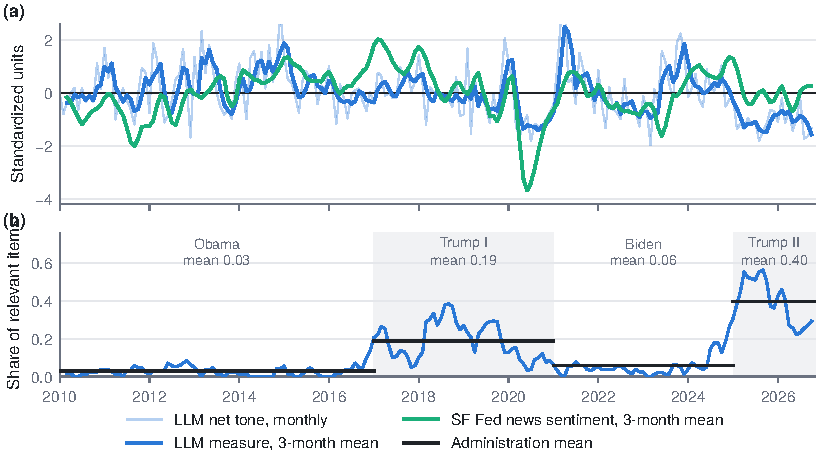
\includegraphics[width=\textwidth]{figures/fig_media.pdf}
  \caption{\textbf{National news measures.} Panel (a): LLM net tone of national coverage and the San Francisco Fed news sentiment index, each standardized over 2010–2026. Panel (b): share of relevant national items that blame the president or administration for economic conditions, with administration means; Trump terms are shaded. Sources: \texttt{features/media\_monthly.csv}, \texttt{features/sffed\_news\_sentiment\_monthly.csv}, \texttt{results/stage2\_bias/attribution\_means.csv}.}
  \label{fig:media}
\end{figure}

\subsection{Bias benchmarks}
\Cref{tab:bias} states, for each dimension, the benchmark that unbiased coverage would satisfy and the result.

\begin{table}[htbp]
\centering
\begin{threeparttable}
\caption{\textbf{Candidate media biases: benchmarks and results for national news, 2010–2026}}
\label{tab:bias}
\footnotesize
\begin{tabularx}{\textwidth}{@{}>{\raggedright\arraybackslash}p{0.13\textwidth} >{\raggedright\arraybackslash}p{0.27\textwidth} X@{}}
\toprule
Dimension & Benchmark & Result\\
\midrule
Tone (negativity) & Equal response to equal-sized good and bad news in unemployment, inflation and GDP releases & Not robust. The joint test rejects symmetry ($p < 0.001$) only because both GDP coefficients are negative, an artifact of the 2020 swings; with lagged tone $p = 0.20$, and without 2020 the asymmetry is positive.\\
Selection and salience & Equal topic elasticities to rises and falls of the same size & Rising-prices coverage responds to rising inflation (0.13) as easing-inflation coverage responds to falling inflation (0.12); difference 0.02 [−0.17, 0.26]. Layoffs versus hiring: 0.029 versus 0.007, difference 0.02 [−0.16, 0.17].\\
Framing & Share of price-level wording should fall once inflation falls & Among price-framed items, level wording fell from 0.76 (2010–2019) to 0.68 before and 0.60 after the 2022 peak. What stayed high is the volume of price coverage: price-framed items rose from 0.25 to 0.47 of relevant items.\\
Factual calibration & Official vintage available on the publication date & National: 2 of 68 checkable claims wrong (2.9\%). Social: 0 of 9 wrong, but 6 of 13 inflation figures without a named measure match no official reading (four are 15–50\% hyperbole).\\
Political attribution & Similar economic conditions under different administrations & Blame share 0.03 (Obama), 0.19 (Trump I), 0.06 (Biden), 0.40 (Trump II); conditional on fundamentals, Trump II $+0.35$ ($p < 0.001$). Not a coder artifact (name swaps), but not proof of bias: tariffs are direct presidential decisions.\\
Across sources & Same months, different outlets & Local news is less negative than NYT and Guardian (net tone $+0.37$ [0.30, 0.44]); so is the Media Cloud national sample ($+0.17$). YouTube comments are more negative ($-0.19$) and more price-focused.\\
\bottomrule
\end{tabularx}
\begin{tablenotes}[flushleft]\footnotesize
\item \textit{Notes:} Regressions of monthly national measures on positive and negative parts of real-time data changes, HAC standard errors; brackets are 95\% bootstrap intervals. Factual claims are parsed by rule and compared with ALFRED vintages; a hand check of 30 parses found 26 correct and the rules were revised. Cross-source differences describe what sources supply and are not called bias.
\item \textit{Source:} \texttt{results/stage2\_bias/}, \texttt{results/stage2\_factcal/}; \texttt{results/FINDINGS\_stage2.md}.
\end{tablenotes}
\end{threeparttable}
\end{table}

National coverage did not overweight bad news relative to equivalent good news; what persisted was the volume of price coverage. Because the 2025–2026 national measure is more negative than local and broader national news, it is, if anything, a generous measure of negative coverage.

% ======================================================================
\section{Does media analysis improve forecasts?}\label{sec:forecast}

M2 adds national net tone for month $t-1$ to M1; M3 adds it to M1c, which is M1 plus the four household variables, a governing-party dummy and a pre-election dummy. The pre-registered primary test is M3 against M1c, the only comparison that asks whether media carry information beyond real pressures and politics. Forecasts are one step ahead from an expanding window (evaluation 2017-01 to 2026-10) with lagged sentiment, a choice fixed before results were seen, and are compared with the Clark–West test \citep{clark2007}.

\Cref{tab:forecast} shows that tone improves on fundamentals alone by a small margin (RMSE ratio 0.991, $p = 0.041$), most clearly in 2017–2019 and 2025–2026. Against M1c it adds nothing (ratio 1.001, $p = 0.23$), and none of 20 registered specifications (the main one and 19 variants) is significant at 5\% ($p$ from 0.065 to 0.85 for the variants; \cref{fig:spec} in \cref{app:robust}), so falsification criterion 2 is triggered. Without lagged sentiment, tone is significant in 18 of the 20, but that model's RMSE is more than twice as large and tone most likely stands in for the persistent part of the gap. The controls themselves worsen out-of-sample accuracy (ratio 1.16), for the extrapolation reasons of \cref{sec:baseline}.

\begin{table}[htbp]
\centering
\begin{threeparttable}
\caption{\textbf{Out-of-sample forecast comparison}}
\label{tab:forecast}
\small
\begin{tabular}{@{}l r c c c c c c@{}}
\toprule
 & & \multicolumn{2}{c}{M2 vs.\ M1} & \multicolumn{2}{c}{M3 vs.\ M1c} & \multicolumn{2}{c}{M1c vs.\ M1} \\
 & & \multicolumn{2}{c}{tone added} & \multicolumn{2}{c}{tone added (primary)} & \multicolumn{2}{c}{controls added} \\
\cmidrule(lr){3-4}\cmidrule(lr){5-6}\cmidrule(l){7-8}
Evaluation period & Months & RMSE ratio & $p$ & RMSE ratio & $p$ & RMSE ratio & $p$ \\
\midrule
2017-01 to 2026-10 & 118 & 0.991 & 0.041 & 1.001 & 0.23 & 1.161 & 0.80 \\
\quad excluding 2020-03 to 2020-12 & 108 & 0.976 & 0.005 & 1.022 & 0.42 & 1.119 & 0.75 \\
2017--2019 & 36 & 0.937 & 0.017 & 0.942 & 0.007 & 1.015 & 0.37 \\
2020--2022 & 36 & 1.023 & 0.48 & 1.018 & 0.52 & 1.258 & 0.75 \\
2023--2024 & 24 & 1.004 & 0.35 & 0.954 & 0.076 & 1.007 & 0.29 \\
2025--2026 & 22 & 0.920 & 0.005 & 0.999 & 0.34 & 1.076 & 0.96 \\
\addlinespace
\textit{2017-01 to 2026-10, no AR term} & 118 & 0.946 & 0.006 & 0.926 & 0.004 & 0.831 & < 0.001 \\
\bottomrule
\end{tabular}
\begin{tablenotes}[flushleft]\footnotesize
\item \textit{Notes:} One-step-ahead recursive forecasts of the ICS from an expanding window starting 2010-06; the first window ends 2016-12. All rows except the last include ICS$_{t-1}$. M1: real-time unemployment, PCE inflation and GDP growth; M1c: M1 plus the four household variables, a governing-party dummy and a pre-election dummy; M2 and M3 add national LLM net tone for month $t-1$. RMSE ratio = larger model / smaller model, so values below 1 favour the larger model. $p$: one-sided Clark--West test with HAC variance.
\item \textit{Source:} \texttt{results/stage3\_forecast/comparisons.csv}.
\end{tablenotes}
\end{threeparttable}
\end{table}




In sample the tone coefficient is positive and stable ($\gamma = 5.03$, s.e.\ 1.40) but small: one standard deviation of monthly tone (about 0.20) is associated with about 1.0 ICS point on impact and 1.8 in the long run. Tone in 2025 was 0.15 below its 2019 mean, about 1.6 points or 4.5\% of the 2025 gap (3.6\% in 2026); in 2021–2024 it was not more negative than in 2019. These are upper bounds on an association. Six secondary media measures, tested with a Benjamini–Hochberg correction \citep{benjamini1995}, all have adjusted $p \geq 0.43$, and the SF Fed index and economic policy uncertainty \citep{baker2016} add nothing. Exploratory: the tone coefficient rises after the July 2024 switch to web interviews ($+11.7$, $p = 0.010$, 28 months).

% ======================================================================
\section{Timing and causal reasoning}\label{sec:causal}

Observational data establish order and association, not effects; hence ``associated with'' and ``precedes'' throughout.

\para{Two-way timing.} Local projections \citep{jorda2005} control for real-time fundamentals, data surprises, event dummies (shutdowns, tariff announcements, bank failures, the pandemic) and lags of both series. Tone is followed by slightly higher sentiment at horizons 0–2 (0.061–0.070 standard deviations, about 0.9 points), but the pre-registered 0–6 average is not significant (0.029, one-sided $p = 0.22$). Sentiment is followed by more positive tone four and five months later (0.34, 0.38; average 0.11, $p = 0.22$). \Cref{fig:lp} shows weak feedback in both directions, not media leading sentiment.

\begin{figure}[htbp]
  \centering
  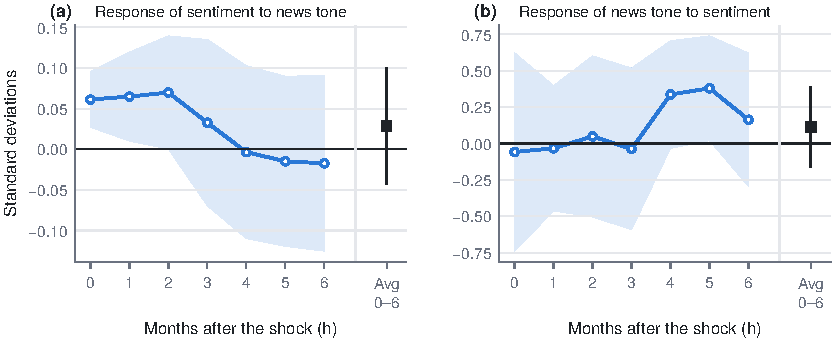
\includegraphics[width=\textwidth]{figures/fig_lp.pdf}
  \caption{\textbf{Local projections in both directions.} Panel (a): response of standardized ICS to a one-unit change in standardized national tone in month $t-1$; panel (b): response of standardized tone to standardized ICS. Bands and bars are 95\% confidence intervals (HAC); the square is the pre-registered average over horizons 0–6. Source: \texttt{results/stage4\_timing/local\_projections.csv}.}
  \label{fig:lp}
\end{figure}

\para{Excess tone.} Relative to a 2010–2019 regression on fundamentals and household variables, tone since 2021 is less negative than predicted (+0.18, $p = 0.011$); for 2025–2026 the residual is zero ($-0.01$, $p = 0.45$), or $-0.15$ with a full-period fit, and fundamentals explain little of tone ($R^2 = 0.06$).

\para{Recall.} Conditional on fundamentals, one unit of higher tone is associated with 45 points fewer respondents recalling unfavorable news (about 9 per standard deviation, $p = 0.001$), and topics match one to one: price coverage predicts recalled price news (17.2, $p < 0.001$) while layoff coverage does not ($-0.5$, $p = 0.85$), and layoff coverage predicts recalled employment news (62.3, $p = 0.031$). Once recalled news enters the ICS equation, tone loses its coefficient ($-1.5$, $p = 0.74$). This ordering is consistent with a path from coverage to recall to sentiment, but recall is explained more by fundamentals (unique $R^2$ 0.21) than by tone (0.14), which triggers falsification criterion 6.

\para{Partisan heterogeneity.} The NYT audience leans Democratic, so an exposure channel should make Democrats' sentiment more sensitive to its tone. It does not: the coefficients are 4.5 for Democrats, 5.5 for independents and 6.8 for Republicans (difference Democrats minus Republicans $-2.3$, $p = 0.57$).

\para{Reverse causality and common shocks.} Pessimistic consumers may seek negative content and publishers may supply it, and an economic shock moves both coverage and sentiment. The controls above address common shocks only partly, and no observational design here separates audience demand from media supply. We therefore propose, rather than claim, a causal design (\cref{app:causal}): a pre-registered randomized experiment in which five arms present the same official figures as a balanced summary, as price levels, as inflation rates, in household terms or as national aggregates, with Michigan's five index questions and one-year inflation expectations as outcomes (394 respondents per arm for $d = 0.2$ at 80\% power; consent, IRB approval, no deception). Local newspaper closures and Sinclair acquisitions \citep{martin2019} offer quasi-experiments for staggered difference-in-differences \citep{callaway2021} if state-level sentiment data were available. Even a clean experimental effect $\tau$ maps into index points only through population weights, exposure and persistence, $\Delta \mathit{ICS} \approx \sum_g w_g e_g \tau_g \rho_g$; with $e = 0.5$, $\tau = 0.1$ standard deviations and $\rho = 0.3$, the national effect would be about 0.2 points.

% ======================================================================
\section{Mechanisms, heterogeneity and the pre-election period}\label{sec:mech}

\para{What the data can measure.} Text establishes framing and selective coverage, not a reader's cognitive bias. \Cref{tab:mech} sorts the four candidate mechanisms by what was measured, what has only compatible evidence and what cannot be measured. Sentiment shows no robust negativity asymmetry: the only significant specification has the opposite sign ($+4.9$, $p = 0.03$) and vanishes without pandemic months ($p = 0.67$). Gasoline and food prices add nothing in 2010–2019 ($p = 0.56$, $0.46$) and reduce the 2025–2026 gap by 2.2\%. The elevated share citing high prices fits anchoring, though part of its rise may reflect the survey-mode change.

\begin{table}[htbp]
\centering
\begin{threeparttable}
\caption{\textbf{Candidate perceptual mechanisms: what the data can and cannot measure}}
\label{tab:mech}
\footnotesize
\begin{tabularx}{\textwidth}{@{}>{\raggedright\arraybackslash}p{0.12\textwidth} >{\raggedright\arraybackslash}X >{\raggedright\arraybackslash}X >{\raggedright\arraybackslash}p{0.17\textwidth}@{}}
\toprule
Mechanism & Measured (aggregate level) & Compatible evidence only & Not measurable here\\
\midrule
Negativity bias & Media: no robust good/bad news asymmetry (\cref{tab:bias}). Sentiment: no robust asymmetry; the only significant sum has the opposite sign & -- & Individual information processing\\
Availability & Price coverage matches recalled price news, with a layoff placebo; gasoline and food add nothing in 2010–2019 & Gasoline is significant in the full sample, which includes gap years & Specific remembered episodes\\
Anchoring to past prices & Cumulative versus 12-month inflation: not identified in 2010–2019 ($p = 0.79$) & Significant in the 2000 window and full sample; ``worse off because of high prices'' 7.3\% (2019), 39.8\% (2022), 44.8\% (2025–26) & Personal reference prices\\
Confirmation bias & Not identifiable & Opposite partisan jumps at changes of administration; partisan gap paths correlate $-0.72$ & Individual beliefs and exposure; proposed experiment\\
\bottomrule
\end{tabularx}
\begin{tablenotes}[flushleft]\footnotesize
\item \textit{Source:} \texttt{results/stage5\_mechanisms/}; \texttt{results/FINDINGS\_stage5.md}.
\end{tablenotes}
\end{threeparttable}
\end{table}

\para{Who is pessimistic.} With each group's own M1 fitted on 2010–2019, the 2025–2026 gap is broad and similar: within each dimension group gaps differ by at most 7.5 points around a level of 32–42 (\cref{fig:groups}). In 2021–2022, by contrast, young, college-educated and northeastern respondents showed almost no gap. Party is the only dimension with large recent differences, and they follow the party in power. Groups with different media diets would be expected to diverge under a media explanation; the uniform recent gap fits that poorly, although the data cannot link group differences to exposure.

\begin{figure}[htbp]
  \centering
  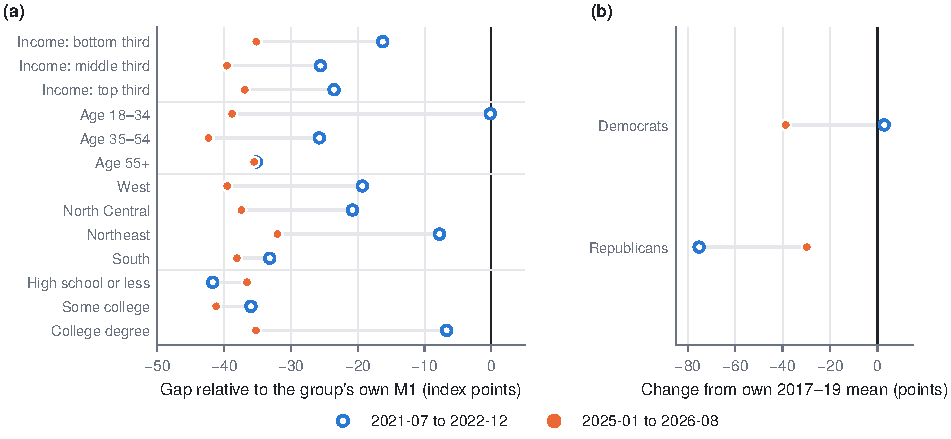
\includegraphics[width=\textwidth]{figures/fig_groups.pdf}
  \caption{\textbf{The gap by group.} Panel (a): mean ICS gap relative to each group's own M1, fitted on 2010–2019. Panel (b): change in partisan ICS relative to each party's own February 2017 to December 2019 mean (party series are not long enough for M1). Sources: \texttt{results/stage5\_mechanisms/group\_gaps\_monthly.csv}, \texttt{results/stage4\_timing/group\_gaps\_monthly.csv}.}
  \label{fig:groups}
\end{figure}

\para{Survey mode.} Within the web-only period, which removes any mode level difference, the ICS gap widened from $-23.0$ (second half of 2024) to $-39.3$ (2026), whereas in the last phone-only stretch it narrowed by 6.7. The mode change cannot explain the recent widening.

\para{Election proximity.} In 2026 the gap was already $-38.8$ in January–April and $-40.4$ in May–October ($-1.6$, against $-0.2$ to $+3.6$ in the 2010–2022 midterm years); pooled pre-election months show no different dynamics (midterm years $+0.60$, $p = 0.22$). Over the same months PCE inflation rose from 2.8\% to 3.7\%, gasoline from \$3.15 to \$4.18 a gallon and the mortgage rate from 6.15\% to 6.61\%, so even a pre-election change could not be attributed to the campaign.

\para{Recent social and local sources.} YouTube comments are more negative than national news but barely track the gap (correlation 0.16, against 0.62 for national news in the same months; local news 0.44 over 19 months; quarterly Reddit 0.10), a descriptive result for these periods only.

% ======================================================================
\section{What would contradict a media-bias explanation?}\label{sec:falsify}

Of the eight pre-registered criteria in \cref{tab:falsify}, two are triggered (no out-of-sample value; recall follows the economy), and two more are not triggered literally but point away from media bias (criteria 1 and 3). \Cref{tab:findings} separates what we found from what remains a hypothesis.

\begin{table}[htbp]
\centering
\begin{threeparttable}
\caption{\textbf{Pre-registered falsification criteria for the media-bias explanation}}
\label{tab:falsify}
\footnotesize
\begin{tabularx}{\textwidth}{@{}r >{\raggedright\arraybackslash}p{0.2\textwidth} >{\raggedright\arraybackslash}X >{\raggedright\arraybackslash}p{0.17\textwidth}@{}}
\toprule
\# & Evidence against media bias & Result & Verdict\\
\midrule
1 & Tone is explained by fundamentals & Residual tone since 2021 $+0.18$ ($p = 0.011$), less negative than predicted; 2025–26 $-0.01$ ($p = 0.45$) & Not triggered; sign contradicts media bias\\
2 & No out-of-sample gain & M3 vs.\ M1c: $p = 0.23$; 0 of 20 specifications significant & \textbf{Triggered}\\
3 & Sentiment leads media & Average 0–6 response $p = 0.22$ in both directions & Not triggered; no media lead either\\
4 & Real pressures explain the gap & Household variables leave the gap unchanged but are not identified & Not triggered (low power)\\
5 & Gap is measurement or partisanship & Mode: ICC $\approx$ 8 points; composition $\leq$ 2.7 points & Not triggered\\
6 & Recall follows the economy & Unique $R^2$: fundamentals 0.21, tone 0.14 & \textbf{Triggered}\\
7 & No difference across groups & Party and age gaps differ, but along partisan lines & Not triggered\\
8 & Measurement is unstable & 0 of 39 excess flip rates significant; three tone measures agree in sign & Not triggered\\
\bottomrule
\end{tabularx}
\begin{tablenotes}[flushleft]\footnotesize
\item \textit{Notes:} Criteria and decision rules were frozen before estimation. For criteria 4 and 5 the pre-registered threshold is half of the gap.
\item \textit{Source:} \texttt{results/FINDINGS\_stage4.md}, section 2.
\end{tablenotes}
\end{threeparttable}
\end{table}

\begin{table}[htbp]
\centering
\begin{threeparttable}
\caption{\textbf{Findings and remaining hypotheses}}
\label{tab:findings}
\footnotesize
\begin{tabularx}{\textwidth}{@{}>{\raggedright\arraybackslash}p{0.2\textwidth} >{\raggedright\arraybackslash}X >{\raggedright\arraybackslash}p{0.27\textwidth}@{}}
\toprule
Question & Finding (supported by this paper's evidence) & Still a hypothesis\\
\midrule
RQ3 Fundamentals & Explain 7–11\% of the decline since 2019; 2025–26 gap $-36$ to $-40$, robust to window and specification (\cref{tab:gap,tab:alt}) & Size of the 2021–22 gap (window-dependent)\\
H1 Real pressures & Not identified in 2010–2019; cumulative inflation explains about a quarter of the gap in an exploratory window & Price-level anchoring as a major cause\\
H3 Measurement, timing & Mode shifts ICC by about 8 points; composition $\leq$ 2.7; gap widened within the web period and predates the campaign & --\\
RQ1 Media bias & LLM coding valid; no coder bias detected; no robust negativity or selection asymmetry; blame share 0.40 under Trump II (\cref{tab:ai,tab:bias}) & Whether the blame shift is bias or accurate attribution\\
RQ5 Forecasting & Small gain over fundamentals only; none after controls (\cref{tab:forecast}) & --\\
RQ2 Impact & Weak two-way association; tone-related share $\leq$ about 5\% of the gap & Effect of framing on beliefs (experiment)\\
RQ4 Mechanisms & Negativity and availability not robust; anchoring and confirmation only compatible (\cref{tab:mech}) & Individual-level mechanisms\\
\bottomrule
\end{tabularx}
\end{threeparttable}
\end{table}

% ======================================================================
\section{Conclusion}\label{sec:conclusion}

Consumer sentiment in 2025–2026 is roughly 36–40 points below what real-time fundamentals predict, and the gap is robust, broad across groups, larger than any plausible mode or composition effect, and in place before the campaign. National news tone is associated with sentiment, but weakly, in both directions, and without forecasting value once household pressure and politics are controlled; national coverage shows no robust negativity or selection bias, and the rise in blame on the administration coincides with direct policy decisions. Media bias, as far as these data can measure it, is not the main explanation of the gap. The remaining sources (the price level itself, policy uncertainty, individual information processing) are hypotheses for future work, not conclusions.

\para{Practical implication.} For forecasting and risk management, the gap should be treated as a persistent state, not as noise around fundamentals or a media artifact that news sentiment can correct. A model mapping Michigan levels to spending or credit risk with pre-2020 relationships \citep{carroll1994} will read 2025–2026 as a much deeper downturn than fundamentals justify. Monitoring the gap with its prediction interval, alongside household-price measures, is more informative than adding a news-tone signal, which does not improve forecasts once those pressures are included.

\para{Limitations.} The analysis is observational and supports statements about order and association only. The national media measure rests on two outlets and about 26 relevant items per month (reliability 0.62), with January and October 2026 incomplete; social and local sources cover only recent periods; the factual-calibration, name-swap and sub-period tests have small samples; household channels cannot be identified in a 2010–2019 window; and exact LLM replication depends on the stored outputs. \textit{Update plan:} the final October Michigan reading (October 23) and advance third-quarter GDP will be added with the same scripts; the November reading arrives after election day and will be reported as a post-election observation.

\para{Ethics.} All data are public or obtained through official interfaces. Author and account fields were never stored, raw text is not redistributed (the package provides identifiers and retrieval scripts, per platform terms), and no AI system served as an annotator. The proposed experiment uses only truthful framings of official data and requires informed consent and IRB approval.

\bibliographystyle{unsrtnat}
\bibliography{references}

% ======================================================================
\clearpage
\appendix
\crefalias{section}{appendix}
\renewcommand{\thesection}{\Alph{section}}
\counterwithin{table}{section}\counterwithin{figure}{section}
\renewcommand{\thetable}{\thesection\arabic{table}}\renewcommand{\thefigure}{\thesection\arabic{figure}}
\section{Data provenance and timing}\label{app:data}

\begin{table}[htbp]
\centering
\begin{threeparttable}
\caption{\textbf{Economic series and timing rules}}
\label{tab:data}
\footnotesize
\begin{tabularx}{\textwidth}{@{}>{\raggedright\arraybackslash}p{0.27\textwidth} >{\raggedright\arraybackslash}p{0.22\textwidth} X@{}}
\toprule
Series & Source & Treatment\\
\midrule
ICS, ICC, ICE; partisan and demographic indices; news-heard and reasons questions & University of Michigan Surveys of Consumers & Monthly, final readings; 2026-10 preliminary. Partisan indices monthly from 2017-02.\\
U-3 unemployment rate (SA) & BLS via ALFRED & Vintage available on the 1st of the survey month.\\
Headline PCE price index & BEA via ALFRED & Year-over-year inflation and 36-month cumulative inflation computed within one vintage.\\
Real GDP & BEA via ALFRED & Latest published quarter, q/q SAAR (y/y as robustness); step function, never interpolated.\\
Mortgage rate, gasoline price & Freddie Mac PMMS, EIA via ALFRED & Never revised; months before the first vintage filled from it.\\
Real disposable income per capita & BEA via ALFRED & From 2010-06, the first available vintage.\\
News sentiment; policy uncertainty & SF Fed; Baker–Bloom–Davis & Robustness only.\\
Events & FOMC, shutdowns, tariffs, bank failures, pandemic & 158 dated events for controls and the dashboard.\\
\bottomrule
\end{tabularx}
\begin{tablenotes}[flushleft]\footnotesize
\item \textit{Source:} \texttt{provenance/}, \texttt{data/processed/econ\_monthly\_realtime.csv}; full documentation in \texttt{README\_data.md}.
\end{tablenotes}
\end{threeparttable}
\end{table}

The ALFRED API is queried for every vintage of each series; each survey month uses the last vintage published before its first day. A robustness check uses Michigan's preliminary release date as the cutoff instead. Two longer windows test extrapolation: 2000-09 to 2019-12 is fully real time, and 1978–2019 is quasi real time (pre-2000 PCE from the earliest vintage, GDP from the Philadelphia Fed real-time data set).

\section{Codebook and prompt}\label{app:codebook}

The human labeling guide (\texttt{annotation/codebook\_v1.md}) defines the unit, the relevance rule and the five dimensions with examples and boundary rules. Tone is coded three times: \texttt{tone\_overall} (wording), \texttt{fact\_direction} (whether the reported facts are good or bad news for households) and \texttt{emotional\_intensity} (0–2). Topics are 13 binary flags. Framing has three independent axes (price level or rate; household or national; current or forecast). Factual calibration records whether a numerical claim is present, its text, and definition errors. Political attribution records up to two actors and whether each receives credit or blame; the guide states that criticism is not bias.

The frozen prompt (\texttt{prompts/label\_prompt\_v2.md}, SHA-256 9f95f20a…) reproduces the codebook, requires a verbatim evidence excerpt for every non-empty label and returns JSON. Annotation sampling (seed 20261015) stratified 360 items by source: NYT 125, Guardian 40, Media Cloud national 15, Media Cloud local 60, Reddit 90 and YouTube 30. The 32 gold items marked relevance ``unsure'' are excluded from relevance precision and recall and reported as a count.

\section{Causal design proposal}\label{app:causal}

\para{Randomized framing experiment.} Five arms show the same month of official data. A (control) states the inflation rate, unemployment rate and GDP growth without comment. B states the cumulative price increase since early 2020. C states the inflation rate and its fall from the 2022 peak. D translates the same figures into monthly household spending. E places them in a national-aggregate narrative. Figures are filled in from the latest releases at fielding and checked by someone not involved in the hypotheses. Outcomes are Michigan's five index questions in original wording and order, scored as Michigan does, and the one-year inflation expectation; secondary outcomes are recall of unfavorable news and a manipulation check. The four comparisons of B–E with A are primary, with Holm correction; 394 respondents per arm detect $d = 0.2$ with 80\% power (about 700 if $d = 0.15$). Estimation is OLS with HC2 errors and pre-specified covariates; heterogeneity by party and self-reported news use is pre-registered. A one-week follow-up on a subsample estimates persistence $\rho$. Online samples are weighted to the CPS.

\para{Quasi-experiments.} (i) Closure of a market's only daily newspaper, and (ii) Sinclair acquisitions, which shift local stations toward national political coverage \citep{martin2019}. Both use staggered difference-in-differences \citep{callaway2021} with pre-trend tests and must address spillovers to national and social media. Both require geographic sentiment data finer than Michigan's four public regions and a local content data set that demonstrates the first stage.

\para{From sample to index.} $\Delta \mathit{ICS} \approx \sum_g w_g e_g \tau_g \rho_g$ requires population weights, population-level exposure estimates (for example, a media-diary panel), transportability of $\tau$ and an additivity assumption for repeated exposure; sensitivity ranges for $\rho$ and aggregation should accompany any estimate. Full text: \texttt{results/CAUSAL\_DESIGN\_PROPOSAL.md}.

\section{Robustness of the forecast tests}\label{app:robust}

\Cref{fig:spec} reports every registered variant of the forecast comparison in \cref{sec:forecast}. Adding tone to fundamentals alone is significant at 5\% in 9 of the 20 specifications; adding it to the controlled model is significant in none.

\begin{figure}[htbp]
  \centering
  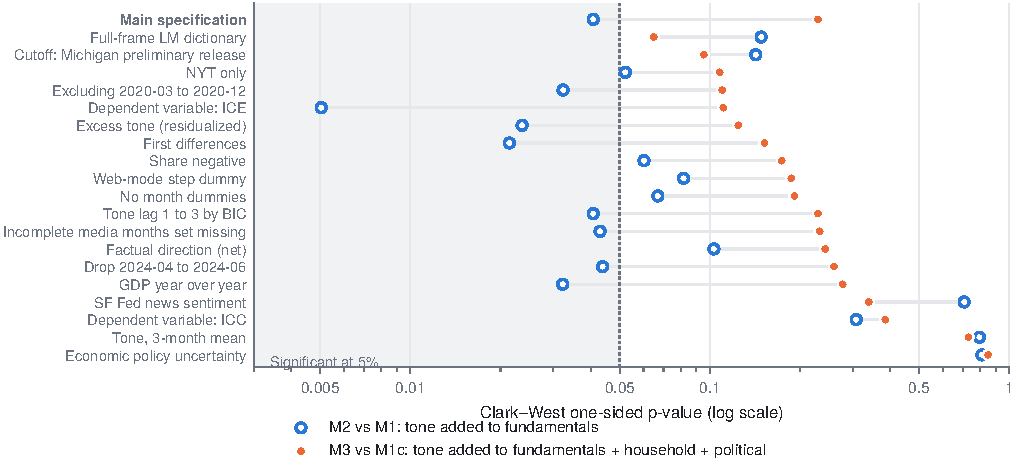
\includegraphics[width=\textwidth]{figures/fig_spec.pdf}
  \caption{\textbf{Specification curve for the media forecast tests.} Clark–West $p$-values for adding lagged national tone (or the alternative media measure named) to fundamentals alone (hollow) and to fundamentals plus household and political controls (filled), AR version. The shaded area marks significance at 5\%. Source: \texttt{results/stage3\_robustness/variants.csv}.}
  \label{fig:spec}
\end{figure}

\section{Reproducibility}\label{app:repro}

\begin{itemize}
  \item \textbf{One command.} \texttt{sh src/process/run\_all.sh} rebuilds the data and corpus from raw files; \texttt{sh src/analysis/run\_research.sh} reruns stages 1–5 deterministically (seed 20261015); \texttt{python3 src/report/make\_figures.py} and \texttt{make\_tables.py} regenerate every figure and the numeric tables in this report from the frozen result files.
  \item \textbf{Registry.} \texttt{results/spec\_registry.csv} lists 150 specifications with their status (pre-registered, robustness, exploratory); \texttt{results/script\_sha256.csv} fixes script versions; \texttt{DECISIONS.md} logs every deviation with its write time.
  \item \textbf{AI outputs.} All LLM outputs, prompts with hashes, run logs and the model declaration are stored under \texttt{labels/ai/}. Because the model cannot be pinned by weights or temperature, the stored outputs, not a re-run, are the reference.
  \item \textbf{Human labels.} Both annotators' raw workbooks, agreement statistics, the adjudication log and the gold standard are in \texttt{labels/} and \texttt{annotation/}.
  \item \textbf{Findings.} \texttt{results/FINDINGS\_stage1.md} to \texttt{FINDINGS\_stage5.md} record each stage's frozen results with the file behind every number.
\end{itemize}

\end{document}
